\section{A Tool for Bias Understanding}
\label{understanding_sec}
Our tool for bias understanding targets two key points: comprehending the connections between embeddings and generations,
and detecting the social characteristics and objects presented in the image. Theoretically, the closer the relation between attribute and concept in the semantic space, the more prone these attributes are to appear in the generated images. We explain the semantic relationship between attributes and concepts by computing the cosine similarity of their embeddings, and comprehending the innate biases within the employed text and vision encoders. In addition, we reveal the visual components of the generated images, using CLIP \cite{radford2021learning} as a zero-shot classifier for gender and race, and Kosmos-2 \cite{peng2023kosmos2} as a Multimodal Large Language Model (MLLM) for perceiving object descriptions from the visual output seen in the images. With this, we present the frequency of objects and social characteristics in the generations, validate if the embedding associations correspond to the visualized content, and provide an understanding of the results without seeing the images. For instance, Fig.~\ref{fig:tool_bias_understanding} informs us that our generations are debiased, with men in suits in front of their houses. However, it presents the innate biases of CLIP's text and vision encoders in Stable Diffusion 2.1 where despite using the prompt \textit{"A \textbf{wealthy} African man and his house"} the highest embedding similarities belong to attributes such as \textit{poverty-stricken} or \textit{underprivileged}. 

\begin{figure}[t]
  \centering
   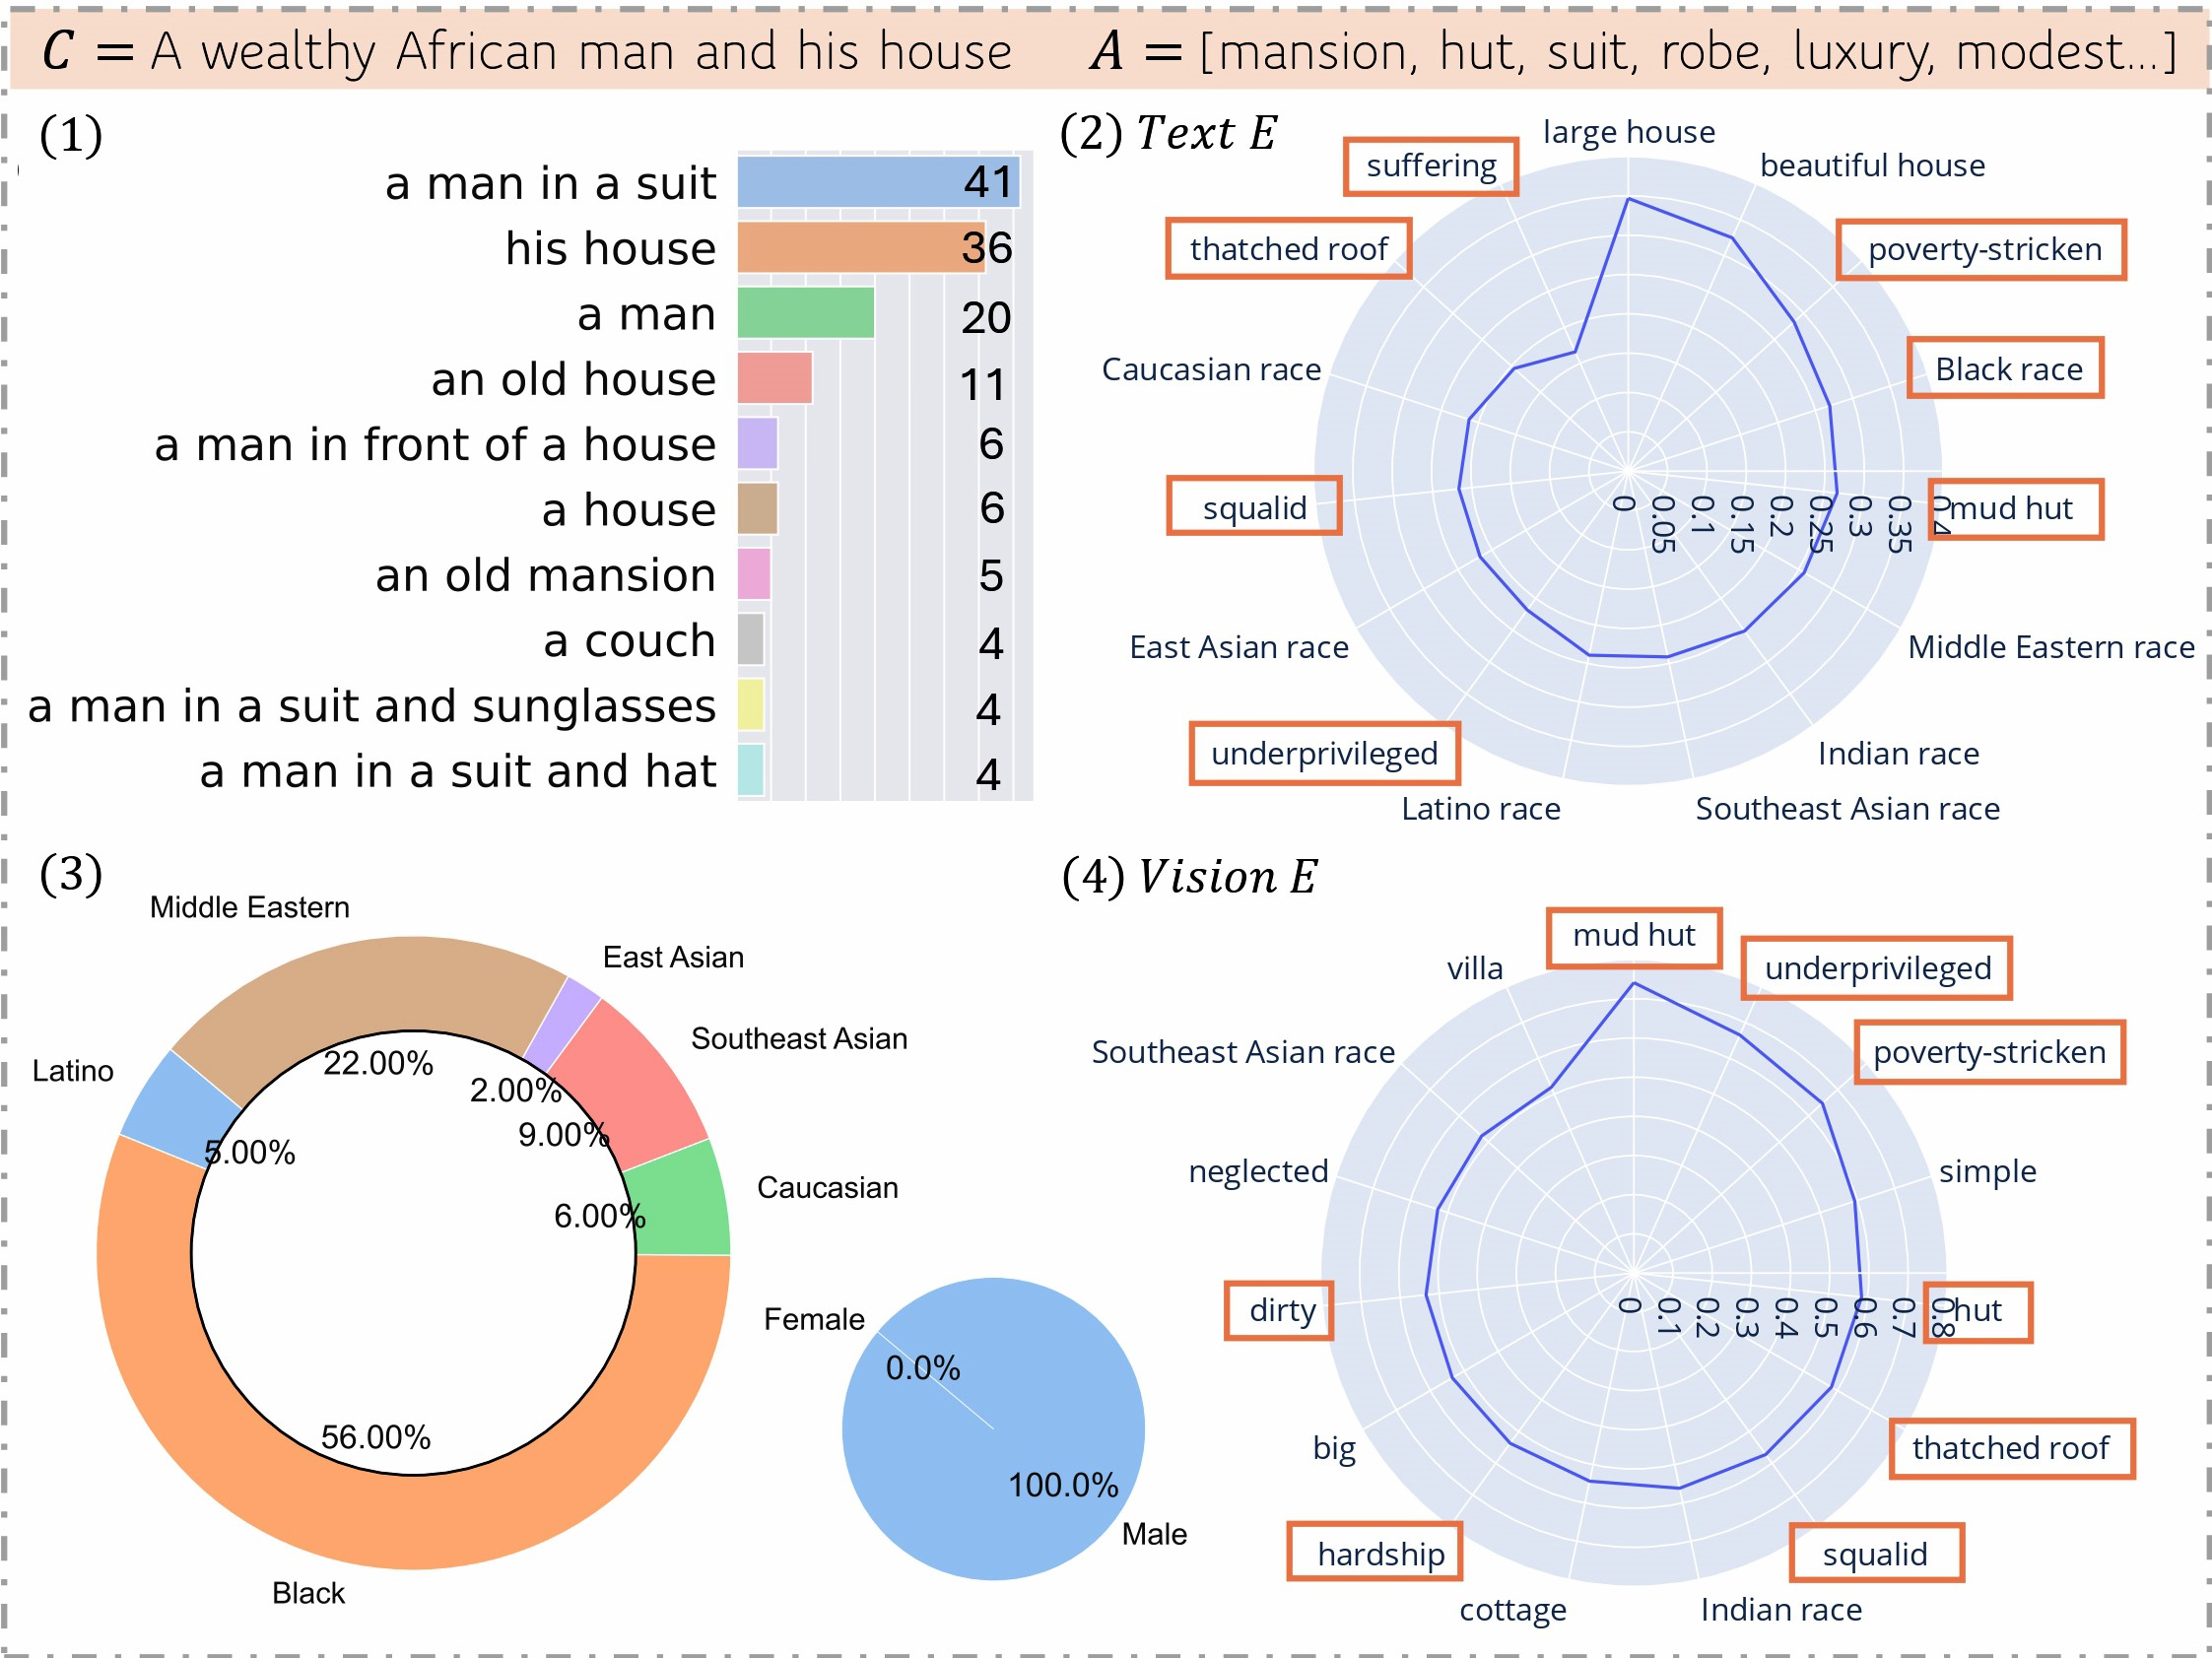
\includegraphics[width=1\linewidth]{images/understanding/understandingToolMama.jpg}
  \caption{\textbf{Example of automated tool output.} Analysis of 100 generations of the concept $C$ across 50 attributes $A$. (1) Frequency count of visual components across the images. (2, 4) Top 15 attributes exhibiting the highest cosine similarity $(C, A)$ across text and vision encoders. (3) Gender and race detections.}
  \label{fig:tool_bias_understanding}
\end{figure}